\documentclass[oneside,12pt]{DISCSthesis}
 \usepackage{graphicx}
% \usepackage{multirow}
 %\usepackage{fancyvrb}
 %\usepackage{rotating}
 \usepackage{longtable}
 \usepackage{pdflscape}
 % \usepackage[justification=centering]{caption}
 %\usepackage[titletoc]{appendix}
 %\usepackage{pdfpages}
\usepackage{setspace}
% \usepackage{enumitem}	\setlist[itemize]{leftmargin=*,itemsep=5pt}
% \usepackage{color,soul} % produces conflicts with
\usepackage{soul}
\usepackage{amsmath}
\usepackage{algpseudocode}
	\renewcommand{\algorithmiccomment}[1]{\hskip0em$\triangleright$ \emph{#1}}
	\renewcommand{\algorithmicrequire}{\hspace*{6pt}\textbf{Input:}}
	\renewcommand{\algorithmicensure}{\hspace*{6pt}\textbf{Output:}}

%\documentclass{article}
\begin{document}
\ThesisAuthor{\textbf{Maria Clara Isabel D. Sia}}
\ThesisTitle{\textbf{Optimizing An Exact Solution to the ($l$, $d$)-Planted Motif Problem}}
\ThesisArea{Computer Science}
\ThesisDefenseYear{2015}
% \DefenseDate{10 July 2013}
% \ThesisGrade{Very Good}

\DepartmentHead{MARLENE M. DE LEON, Ph.D.}
\SchoolHead{EVANGELINE P. BAUTISTA, Ph.D.}
\ThesisAdviser{PROCESO L. FERNANDEZ, JR., Ph.D.}
\FirstPanelMember{XXX, Ph.D.}
\SecondPanelMember{XXX, Ph.D.}
\ThirdPanelMember{XXX, Ph.D.}

\ThesisStyle{MS}{Draft}{-10pt}{15pt}
% Choices for the 1st argument: MS, PhD
% Choices for the 2nd argument: Final, FinalWithCorner, Draft

\FrontMatter
% \input{acknowledgements}

\begin{abstract}
	DNA motif finding is widely recognized as a difficult problem in computational biology and computer science. Because of the usual large search space involved, exact solutions typically require a significant amount of execution time before discovering a motif of length $l$ that occurs in an input set $\{S_{1} ,...,S_{n}\}$ of sequences, allowing for at most $d$ substitutions. 

	This study implements a novel optimization to EMS-GT, a motif search algorithm which operates on a compact bit-based representation of the search space. The optimization takes advantage of distance-related patterns in the search space, in order to speed up the bulk bit-setting operations performed by the algorithm. A Java implementation
	% ---run on synthetic datasets for various challenge instances of the ($l,d$) planted motif problem---
	is shown to be highly competitive against PMS8 and qPMS9, two current state-of-the-art exact algorithms. EMS-GT works extremely well for problems involving short motifs, outperforming both competitors for challenge instances with ($l,d$) values (9,2), (11,3), (13,4) and (15,5), showing runtime reductions of 76\%, 81\%, 77\% and 37\% respectively for these instances, while ranking second to qPMS9 for challenge instance (17,6).
	\end{abstract}

\tableofcontents
\listoffigures
\listoftables

\MainMatter

\chapter{Introduction}
	%section{Start of the intro}
		DNA motif finding is widely recognized as a difficult problem in computational biology and computer science. Motifs are sequences that occur repeatedly in DNA and have some biological significance \cite{das2007survey}; a motif might be a transcription factor binding site, a promoter element, a splicing site, or a marker useful for classification. There are many variants of motif finding problem in the literature. Some look for a motif that repeatedly occurs in a single sequence. Others look for a motif that occurs over some or all of a set of DNA sequences \cite{dasari2010efficient}. One of the latter type is the planted motif problem.\newline

		\begin{figure}[h] \label{fig:example}
			\centering
			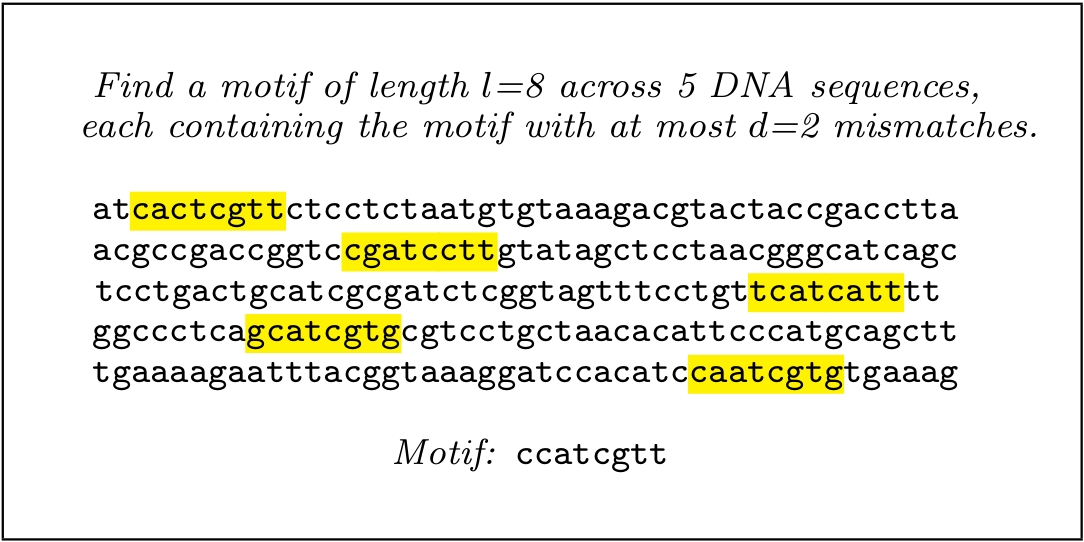
\includegraphics[width=5.5in]{img/example}
			\caption{Sample instance of the planted motif problem.}
			\end{figure}

		The planted motif problem simply asks: ``\emph{Given a set of DNA sequences, can we find an unknown motif of length $l$ that appears at different positions in each of the sequences} \cite{pevzner2000combinatorial}?'' Initially it seems an exhaustive string search will suffice for this problem. However, due to biological mutation, motif occurrences in DNA are allowed to differ from the original motif by up to $d$ characters. This greatly impacts complexity: two distinct variants of a motif---both counting as valid occurrences of the motif---might differ in as many as 2$d$ characters! Brute-force solutions quickly become infeasible as values of $l$ and $d$ increase. All of this shows why ($l$, $d$)-motifs are sometimes called ``subtle'' signals in DNA  \cite{pevzner2000combinatorial}, and why finding them is difficult and computationally expensive. In fact, the motif finding problem has already been shown to be NP-complete \cite{pms2014}. 

		% This study is concerned  optimization to EMS-GT \cite{nabos2015dissertation}, an existing algorithm that solves the planted motif problem for any arbitrary instance up to $l$=17. EMS-GT (short for \emph{Exact Motif Search - Generate and Test}) operates on a compact bit-based representation of the motif search space. This study investigates the properties of Hamming distance-based patterns that appear in the bit-based representation, and evaluates an optimization that takes advantage of these patterns to speed up t.


		This study is concerned with the EMS-GT (\emph{Exact Motif Search - Generate and Test}) algorithm \cite{nabos2015dissertation}, which solves the planted motif problem for any arbitrary instance up to $l$=17. This study investigates Hamming distance-based patterns found to appear in EMS-GT's bit-based representation of the motif search space, and exploits these patterns in a novel optimization for EMS-GT.

	\section{Context of the Study}
		This section formally defines the planted motif problem. It also defines key terms used throughout this paper in discussing exact motif-search algorithms.

		\noindent\textbf{\boldmath DEFINITION 1. $l$-mer, Hamming distance, $d$-neighborhood}

		\noindent An \textbf{\boldmath $l$-mer} is a sequence of length $l$. Given a sequence $S$ of length $L > l$, the $i^{th}$ $l$-mer in $S$ starts at the $i^{th}$ position. The \textbf{\boldmath Hamming distance $dH$} between two $l$-mers of equal length is the number of characters that differ between them. ``Distance'' refers to Hamming distance in this paper, unless otherwise stated.
		\newline\hspace*{35pt} Ex. If $l$ = 5, the second $l$-mer in \texttt{gattaca} is \texttt{attac}.
		\newline\hspace*{55pt} $dH(\texttt{gattaca}, \texttt{cgttaga}) = 3$.

		\noindent The \textbf{\boldmath $d$-neighborhood of an $l$-mer $x$} is the set {\boldmath $N(x, d)$} of all $d$-neighbors of $x$: all $l$-mers $x'$ whose Hamming distance from $x$ is at most $d$, i.e., {\boldmath $dH (x, x') \leq d$}. 
		Meanwhile, the \textbf{\boldmath $d$-neighborhood of a sequence $S$} of length $L > l$ is the set {\boldmath $\mathcal{N}(S, d)$} of all $d$-neighbors of all the $l$-mers in $S$.
		\newline\hspace*{35pt} Ex. \texttt{gatct}, \texttt{cctta}, and \texttt{aatta} are all in $N(\texttt{gatta}, 2)$.
		\newline\hspace*{55pt} For $l$ = 5,
			$\mathcal{N}(\texttt{gattaca}, 2) 
					= N(\texttt{gatta}, 2) \cup 
						N(\texttt{attac}, 2) \cup
						N(\texttt{ttaca}, 2)$.\newline
		
		\noindent\textbf{\boldmath DEFINITION 2. ($l,d$) Planted Motif Problem}
		\newline We formally define the ($l$,$d$) planted motif problem as follows:\bigskip

		\noindent\hspace*{50pt} Given a set $\mathcal{S} = \{S_{1},...S_{t}\}$ of $n$ DNA sequences of length $L$,
		% \newline \hspace*{52pt} the motif length $l$, and the number of allowable mismatches $d$,
		\newline \hspace*{50pt} find $M$, the set of sequences (or motifs) of length $l < L$
		\newline \hspace*{50pt} which have at least one $d$-neighbor in each sequence in $S$. %in $S$.
		
	\section{Objectives of the Study}
		The main objective of this study is to improve the performance of the EMS-GT algorithm. Specifically, it aims:
		\begin{enumerate}
		\item To develop an optimization for EMS-GT that takes advantage of distance-related patterns in the motif search space.
		\item To evaluate the resulting optimization with regard to improvement in runtime and solvable problem instances.
		\item To evaluate the optimized version of EMS-GT against state-of-the-art motif search algorithms.
		\end{enumerate}

	\section{Research Questions}
		This study aims to answer the question: How can the performance of the EMS-GT algorithm be improved?
		Specifically, it aims to answer the following:

		\begin{enumerate}
		\item How can distance-related patterns observed within the motif search space be exploited in an optimization for EMS-GT?
		\item What performance improvement does a pattern-based optimization produce, with regard to runtime and solvable problem instances?
		\item How does the optimized version of EMS-GT compare with state-of-the-art motif search algorithms?
		\end{enumerate}

	\section{Significance of the Study}
		Motif finding is a key problem in 

		Optimizing an exact motif search algorithm, especially one which is competitive with the known state-of-the-art, improves a viable option for real-world motif finding applications. The properties of distance-related patterns within an organized search space, as investigated in this paper, may also prove useful in solving other types of search problems and Hamming distance-related problems.

	\section{Scope and Limitations of the Study}


\chapter{Review of Related Literature}
	Motif finding is a well-studied problem in computing. Various motif search algorithms have been developed,
	falling into two categories: \emph{heuristic} and \emph{exact}. This section gives an overview of algorithms
	of both types, and provides an in-depth description of the exact algorithm EMS-GT.
	
	\section{Heuristic Algorithms}
		Heuristic algorithms perform an iterative local search, for instance by repeatedly refining an input sampling or projection until a motif is found. Gibbs sampling \cite{lawrence1993detecting} and Expectation Maximization (EM), used in the motif-finding tool MEME \cite{lawrence1990expectation,bailey1995unsupervised} both use probabilistic computations to optimize an initial random alignment. (An alignment is simply a set $\{a_{1}, a_{2},...,a_{n}\}$ of $n$ positions, which predicts that the motif occurs at position $a_{i}$ in the given sequence $S_{i}$.) Gibbs sampling tries to refine the alignment one position at a time; %in contrast,
		EM may recompute the entire alignment in a single iteration. Projection \cite{blanchette2002discovery} combines a pattern-based approach with EM's probabilistic approach, trying to guess every successive character of a tentative motif and using EM to verify its guesses. GARPS \cite{huo2009combining} uses a random version of projection, in tandem with the Genetic Algorithm (GA), for yet another iterative approach. These are just some of many successful heuristic algorithms.

	\section{Exact Algorithms}
		Heuristic approaches are non-exhaustive and thus not always guaranteed to find a solution. Exact algorithms, on the other hand, perform an exhaustive search of possible motifs and so always find the planted motif.

		WINNOWER \cite{pevzner2000combinatorial} and its successor MITRA \cite{eskin2002finding} are exact algorithms that look at pairwise $l$-mer similarity to find motifs. In a set of DNA sequences, there are numerous pairs of ``similar'' $l$-mers, which come from different sequences and have Hamming distances of at most 2$d$ from each other (meaning that they could be two $d$-neighbors of the same $l$-mer). WINNOWER represents these pairs in a graph, with $l$-mers as nodes and edges connecting $l$-mer pairs. It then prunes the graph to identify ``cliques'' of pairs that indicate a motif. MITRA refines this graph representation into a mismatch tree containing all possible $l$-mers, organized by prefix. The tree structure allows MITRA to eliminate entire branches at a time, making it faster than WINNOWER at removing the spurious edges that are not part of any motif clique.

		The current state-of-the-art in exact motif search is qPMS9, the most recent in a series \cite{pms2007,pms2014,pms2015} of Planted Motif Search algorithms. It performs a sample-driven step, which generates a $k$-tuple of $l$-mers from each of $k$ input strings, followed by a pattern-driven step, which generates the common $d$-neighborhood of the tuple and then checks whether any of the $l$-mers in this common neighborhood is a motif. To identify neighbors, qPMS9 efficiently traverses the tree of all possible $l$-mers, using certain pruning criteria explored by predecessors PMSPrune and qPMS7 \cite{pms2007} to quickly discard non-neighbor branches. Sampling in qPMS9 is an improvement on its predecessor PMS8 \cite{pms2014}; in building a $k$-tuple, qPMS9 intelligently prioritizes $l$-mers that have fewer matches with the $l$-mers already selected, such that the common $d$-neighborhood becomes smaller and thus faster to check through.  Finally, both PMS8 and qPMS9 have been implemented to run on multiple processors, allowing them to solve problem instances with ($l, d$) as large as (50, 21) in a few hours.

	\newpage
	\section{EMS-GT}
		EMS-GT \cite{nabos2015dissertation} is an exact motif search algorithm based on the candidate generate-and-test principle.
		It operates on a compact bit-based representation of the search space, identifying the common $d$-neighbors of the $n$ given DNA sequences as motifs. The main idea of EMS-GT is to narrow down the search space to a small set of ``candidate'' motifs based on the first $n'$ sequences, then do a brute-force search for each candidate on the remaining $(n - n')$ sequences to confirm whether or not it is a motif. 
		EMS-GT's approach proceeds in two main steps:
		\begin{enumerate} %[label={\em (\alph*)}]
			\item {\em Generate candidates}\newline
			This step takes the intersection of the $d$-neighborhoods of the first $n'$ sequences $S_{1},S_{2},...,S_{n'}$. Every $l$-mer in the resulting set $C$ is a candidate motif.
				\begin{equation} C = \mathcal{N}(S_{1}, d) \cap \mathcal{N}(S_{2}, d) \cap...\cap \mathcal{N}(S_{n'}, d). \end{equation}
			\item {\em Test candidates}\newline
			This step simply checks each candidate motif $c$ in $C$, to determine whether a $d$-neighbor of $c$ appears in all of the remaining sequences $S_{n'+1},S_{n'+2},...,S_{n}$. If this is the case, $c$ is accepted as a motif in set $M$.
				\begin{equation} M = C \cap \mathcal{N}(S_{n'+1}, d) \cap...\cap \mathcal{N}(S_{n}, d). \end{equation}
			\end{enumerate}

		\newpage{\setstretch{1.0}
		\noindent\hspace*{6pt}{\bf Algorithm 2.1} \textsc{Exact Motif Search - Generate and Test}\small
		\begin{algorithmic}[1] \label{alg:EMS-GT}
			\Require set $S = \{S_{1},S_{2},...,S_{n}\}$ of $L$-length sequences, \newline \hspace*{25pt}motif length $l$, allowable mismatches $d$
			\Ensure set $M$ of candidate motifs %\vspace*{6pt}
			% \State 
			\State $C \leftarrow \{\}$										\hspace*{200pt}\Comment{generate candidates}
			\State $\mathcal{N}(S_{1},d) \leftarrow \{\}$
			\For{$j \leftarrow 1$ to $L-l+1$}
				\State $x \leftarrow j^{th} l$-mer in $S_{1}$
				\State $\mathcal{N}(S_{1},d) \leftarrow \mathcal{N}(S_{1},d) \cup N(x,d)$
			\EndFor
			\State $C \leftarrow \mathcal{N}(S_{1},d)$
			\For{$i \leftarrow 2$ to $n'$}
				\State $\mathcal{N}(S_{i}, d) \leftarrow \{\}$
				\For{$j \leftarrow 1$ to $L-l+1$}
					\State $x \leftarrow j^{th} l$-mer in $S_{1}$
					\State $\mathcal{N}(S_{i},d) \leftarrow \mathcal{N}(S_{i},d) \cup N(x,d)$
				\EndFor
				\State $C \leftarrow C \cap \mathcal{N}(S_{i},d)$
			\EndFor
			\State $M \leftarrow \{\}$										\hspace*{200pt}\Comment{test candidates}
			\For{each $l$-mer $u$ in $C$}
				\State $isMotif \leftarrow$ true
				\For{$i \leftarrow (n'+1)$ to $n$}
					\State $found \leftarrow$ false
					\For{$j \leftarrow 1$ to $L-l+1$}
						\State $x \leftarrow j^{th} l-$mer in $S_{i}$
						\If{$dH(x,u) \leq d$}
							\State $found \leftarrow$ true
							\State break
						\EndIf
					\EndFor
					\If{!$found$}
						\State $isMotif \leftarrow$ false
						\State break
					\EndIf
				\EndFor
				\If{$isMotif$}
					\State $M \leftarrow M \cup u$
				\EndIf
			\EndFor
			\State\Return $M$
			\end{algorithmic}
		}


		\noindent In practice, EMS-GT must perform speedy operations on an array of bits representing the entire motif search space. Subsections 2.3.1 to 2.3.4 discuss the efficient strategies EMS-GT uses for key tasks such as representing sets in the search space, determining whether $l$-mers are neighbors, and generating all neighbors for a given $l$-mer.

		\subsection{Bit-based set representation and $l$-mer enumeration}
			The motif search space consists of the $4^{l}$ possible $l$-mers that can be formed from the nucleic alphabet \{\texttt{a}, \texttt{g}, \texttt{c}, \texttt{t}\}. To efficiently represent sets---such as a $d$-neighborhood, or a set of candidate motifs---within this space, EMS-GT assigns each of the $4^{l}$ $l$-mers a bit flag in an array, set to 1 if the $l$-mer is a member of the set and 0 otherwise. Bit flags correspond to $l$-mers via a simple mapping: EMS-GT maps an $l$-mer $s$ to a bit flag index $x$ by replacing each character with 2 bits (\texttt{a=00}, \texttt{c=01}, \texttt{g=10}, \texttt{t=11}). Note that this mapping scheme enumerates $l$-mers in strict alphabetical order.

			\noindent \hspace*{40pt}{\small Ex. \texttt{tacgt} maps to \texttt{1100011011} = 795; thus, its flag is the $795^{th}$ bit in the array.
				% \hspace*{58pt} Thus, the flag for \texttt{tagct} is bit 795 in the array.}

		\subsection{Bit-array compression}
			EMS-GT's implementation compresses the required set-representation array of $4^{l}$ bits into an equivalent array of $\frac{4^{l}}{32}$ 32-bit integers. The $x^{th}$ bit is now found at position ($x$ mod 32) of the integer at array index $\frac{x}{32}$.\newline
			\hspace*{40pt}{\small Ex. \texttt{tacgt} maps to \texttt{1100011011} = 795 in decimal.\newline
				\hspace*{58pt} \emph{array index}  = $\frac{795}{32}$ = 24 , \hspace*{5pt} \emph{bit position} = 795 mod 32 = 27;\newline %\newline\hspace*{58pt} 
				\hspace*{58pt}Thus, the flag for \texttt{tacgt} is the 27$^{th}$ bit of the integer at array index 24.}
			% \begin{figure}[h] \label{fig:bitarray_demo}
			% 	\end{figure}

		\subsection{XOR-based Hamming distance computation}
			The mapping of $l$-mers to binary numbers  is also useful for computing Hamming distances. An exclusive OR (XOR) bitwise operation between the mappings of two $l$-mers will produce a nonzero pair of bits at every mismatch position; counting these nonzero pairs of bits in the XOR result gives us the Hamming distance. See Algorithm 2.2 for the implementation.\newline
			\noindent\hspace*{40pt} {\small Ex.	\texttt{tacgt} maps to \texttt{1100011011} \newline
				\vspace*{2pt}\hspace*{62pt} \texttt{ttcgg} maps to \texttt{1111011010} \newline				
				\hspace*{62pt}	XOR produces \hspace*{3pt}\texttt{00\hl{11}0000\hl{01}} = 2 mismatches.}

		\subsection{Recursive neighborhood generation}
			To generate a $d$-neighbor of an $l$-mer $x$, we choose $d' \leq d$ positions from 1, 2,..., $l$-1, $l$ and change the character at each of the $d'$ positions in $x$. EMS-GT uses a recursive procedure (Algorithm 2.3) to do this, effectively (1) traversing the tree of all $d$-neighbors and (2) setting the bit flag in the neighborhood array $N$ for each neighbor it encounters. Since we choose up to $d$ positions in the $l$-mer, and have 3 possible substitute characters at each position, the size of the neighborhood $N(x,d)$ is given by: %\bigskip \hspace*{20pt}
			\begin{equation}
				|N(x,d)| = \sum_{i=0}^d \binom{l}{i} 3^{i}
			\end{equation}

		\newpage
		{\setstretch{1.0}
			\noindent \hspace*{6pt}{\bf Algorithm 2.2} \textsc{Hamming distance computation}\small
			\begin{algorithmic}[1]\label{alg:hamming-distance-comp}
				\Require $l$-mer mappings $u$ and $v$
				\Ensure $dH(u,v)$\vspace*{6pt}

				\State $dH(u,v) = 0$
				\State $z \leftarrow u ^ v$
				\For {$i \leftarrow 1$ to $l$}
				\If{$z$ \& 3 != 0}
				\State $dH(u,v) \leftarrow dH(u,v) + 1$
				\EndIf
				\State $z \leftarrow z >>$ 2
				\EndFor
				\State\Return $dH(u,v)$
				\end{algorithmic}
			}

			\bigskip\bigskip\bigskip

		{\setstretch{1.0}
			\noindent \hspace*{6pt}{\bf Algorithm 2.3} \textsc{Recursive neighborhood generation}\small
			\begin{algorithmic}[1]
				\label{alg:recursive-nbr-gen}
				\Require DNA sequence $S$, motif length $l$, mismatches $d$
				\Ensure bit-array $\mathcal{N}$ representing $\mathcal{N}(S,d)$ \vspace*{6pt}
				% \For{$i \leftarrow$ 1 to $4^{l}$}
				\State $\mathcal{N}[lmer] \leftarrow 0,\ \ \forall\ lmer \in $ search space 
				% \EndFor
				\For{each $l$-mer $x$ in $S$}
				\State \textsc{AddNeighbors}($x$, 0, $d$) \hspace*{79pt}\Comment{recursive procedure}
				\EndFor
				\newline
				\State \Comment{make $d$ changes in $l$-mer $x$, from position $s$ onward}
				\Procedure{AddNeighbors}{$x$, $s$, $d$}
					\For{$i \leftarrow s$ to $l$}
						\State $\Sigma' \leftarrow$ \{\texttt{a}, \texttt{g}, \texttt{c}, \texttt{t}\} $- x_{i}$ \hspace*{79pt}\Comment{\small remove $i^{th}$ character of $x$}
						\For{$j \leftarrow 1$ to $|\Sigma'|$}
							\State $neighbor \leftarrow concatenate(x_{1...i-1},\Sigma_{j},x_{i+1...l})$
							\State $\mathcal{N}[neighbor] \leftarrow 1$
							\If{$d > 1$ and $i < l$}
								\State \textsc{AddNeighbors}($neighbor$, $i+1$, $d-1$)
							\EndIf
						\EndFor
					\EndFor
				\EndProcedure
				\State\Return $\mathcal{N}$
				\end{algorithmic}
			}

	% \section{Block-based patterns in Hamming distances}
		% 	We can represent the neighborhood $N(x,d)$ of an $l$-mer $x$ as an array $N$ of $4^{l}$ bit flags, set to 1 if the corresponding $l$-mer is a neighbor and 0 otherwise.
			
		% 	\begin{equation*}
		% 		N_{x'} = \left\{
		% 		\begin{array}{rl}
		% 			1 & \text{if } dH(x,x') \leq d,\\
		% 			0 & \text{otherwise.}%\text{if } dH(x,x') > d.
		% 		\end{array} \right.
		% 		\text{ for any $l$-mer }x'.
		% 		\end{equation*}

		% 	\noindent If we divide $N$ into consecutive blocks of $4^{k}$ flags each, for some {\bf\boldmath block degree $k$}, $0 < k < l$, each block will conform to at most $(k+2)$ bit patterns. We explain that this is due to the alphabetical enumeration of $l$-mers followed in $N$.

		% 	\subsection{Additive property of Hamming distances}
		% 		\noindent Consider $N$ for a certain $l$-mer $x = yz$, where $y$ is the {\bf prefix} (first $l-k$ characters) of $x$, and $z$ is the {\boldmath\bf $k$-suffix} (last $k$ characters) of $x$.
		% 		\vspace{3mm}\newline
		% 		\hspace*{50pt} Ex. For $k$ = 5,\ \ $x$ = \texttt{acgtacgtacgt} $\rightarrow$\ \  $y$ = \texttt{acgtacg}, $z$ = \texttt{tacgt}.
		% 		\vspace{3mm}


				
		% 		\noindent We can infer that the distance between two $l$-mers is the sum of the distance between their prefixes and the distance between their suffixes; thus the distance between $x$ and any other $l$-mer $x'=y'z'$ is given by:
		% 		\vspace{-5mm}
		% 		\begin{equation} dH(x,x') = dH(y,y') + dH(z,z') \end{equation}
		% 		\noindent This means we can redefine the criteria for setting a bit in $N$:
		% 		\begin{equation*}
		% 				N_{x'} = \left\{
		% 				\begin{array}{rl}
		% 					1 & \text{if } dH(y,y') + dH(z,z') \leq d,\\
		% 					0 & \text{otherwise.}%\text{if } d_{y'} + \mathcal{D}(z)_{z'} > d.
		% 				\end{array} \right.
		% 				\text{ for }x' = y'z'.
		% 				\end{equation*}
		% 	\subsection{Alphabetical enumeration scheme}

\chapter{Methodology}
	This section briefly describes procedures for comparing the performance of EMS-GT (including the optimization) and state-of-the-art algorithms.

	\section{Datasets}
		Synthetic datasets were created using a DNA sequence generator written in Java. Each nucleotide character in a sequence is randomly generated; \{\texttt{a}, \texttt{g}, \texttt{c}, \texttt{t}\} each have a 25\% chance of being selected, independent from other characters in the sequence.
		The motif is then planted at a random position in the sequence. As prescribed in \cite{pevzner2000combinatorial} every dataset contains 20 DNA sequences each 600 bases long, with an ($l$, $d$) motif planted exactly once in each sequence.

	\section{Implementation}
		Thee Java implementation of EMS-GT operates on a compact, bit-based enumerative representation of the motif search space. 
		Since a significant part of runtime is spent locating and setting bits in this bit-based representation, optimizations were explored for the bit-setting portion of the algorithm. Investigation of some Hamming distance-based patterns in the search space led to the development and integration of a bit-masking speed-up technique, which exploits these patterns to set bits in entire blocks.

	\section{Evaluation}
		EMS-GT was compared to known state-of-the-art algorithms PMS8 and qPMS9 by benchmarking their performance on challenging instances of the 
		($l, d$) planted motif problem. An ($l$, $d$) problem instance is defined to be a challenging instance if $d$ is the largest value for which the expected number of $l$-length motifs that would occur in the input by random chance does not exceed some limit---typically 500 random motifs \cite{pms2015}. The specific challenge instances used were (9,2), (11,3), (13,4), (15,5), and (17,6), as identified in \cite{pms2015,pms2007}. 
		\bigskip

\chapter{Results and Analysis}
	\section{Pattern-based optimization for EMS-GT}
	
		\newpage{\setstretch{1.0}\small
			\noindent \hspace*{6pt}{\bf Algorithm 4.1} \textsc{Block-based neighborhood generation}\vspace*{6pt}
			\begin{algorithmic}[1]\label{alg:block-nbr-gen}
				\Require DNA sequence $S$, motif length $l$, mismatches $d$
				\Ensure bit-array $\mathcal{N}$ representing $\mathcal{N}(S,d)$ \vspace*{6pt}
				\Comment{compute }

				% \For{$i \leftarrow$ 1 to $4^{l}$}
				\State $\mathcal{N}[lmer] \leftarrow 0,\ \ \forall lmer \in $ search space 
				% \EndFor
				\For{each $l$-mer $x$ in $S$}
				\State $y \leftarrow x_{1...l-k}$ 
				\State \textsc{SetBlocks}($y$, 0, $d$) \hspace*{9pt}\Comment{recursive procedure}
				\EndFor
				\State \Comment{make $d$ changes in prefix $y$, from position $s$ onward}
				\Procedure{SetBlocks}{$x$, $s$, $d$}
					\For{$i \leftarrow s$ to $l$}
						\State $\Sigma' \leftarrow$ \{\texttt{a}, \texttt{g}, \texttt{c}, \texttt{t}\} $- x_{i}$ \hspace*{4pt}\Comment{\small remove $i^{th}$ character in $x$}
						\For{$j \leftarrow 1$ to $|\Sigma'|$}
							\State $neighbor \leftarrow concatenate(x_{1...i-1},\Sigma_{j},x_{i+1...l})$
							\State $\mathcal{N}[neighbor] \leftarrow 1$
							\If{$d > 1$ and $i < l$}
								\State \textsc{AddNeighbors}($neighbor$, $i+1$, $d-1$)
							\EndIf
						\EndFor
					\EndFor
				\EndProcedure
				\State\Return $\mathcal{N}$
				\end{algorithmic}

			}\newpage

		% HUGE WALL OF COMMENT TEXT
			% We can represent the neighborhood $N(x,d)$ of an $l$-mer $x$ as an array $N$ of $4^{l}$ bit flags, set to 1 if the corresponding $l$-mer is a neighbor and 0 otherwise.
			% \begin{equation*}
			% 	N_{x'} = \left\{
			% 	\begin{array}{rl}
			% 		1 & \text{if } dH(x,x') \leq d,\\
			% 		0 & \text{otherwise.}%\text{if } dH(x,x') > d.
			% 	\end{array} \right.
			% 	\text{ for any $l$-mer }x'.
			% 	\end{equation*}\newline		
			% We find that if we divide this bit array $N$ into consecutive blocks of $4^{k}$ flags each, for some $k$, $0 < k < l$, each block will conform to one of at most ($k + 2$), possible bit patterns. We exploit this regularity in order to generate $N$ in blocks.
			% Say we wish to generate $N(x,d)$ for some $l$-mer $x$. We perform the following steps:

			% \begin{enumerate}
			% 	\item We select a value for the {\bf\boldmath block degree $k$}, and divide $x$ into its {\boldmath\bf prefix $y$} (first $l-k$ characters) and its {\boldmath\bf $k$-suffix $z$} (last $k$ characters).\newline
			% 	{\small\hspace*{40pt}Ex. Choose $k$ = 5;\ \ $x$ = \texttt{acgtacgtacgt} $\rightarrow$ \ \  $y$ = \texttt{acgtacg} and $z$ = \texttt{tacgt}.}
			% 	% \newline\hspace*{58pt}divides into }\newline\newline

			% 	\item We generate the {\boldmath\bf distribution $\mathcal{D}(z)$} of Hamming distances from $z$ to all $4^{k}$ possible $k$-suffixes, in which $\mathcal{D}(z)_{z'} = dH(z,z')$ for any $k$-suffix $z'$.

			% 	\item For a given block in $N$, we compute the {\boldmath\bf prefix distance $d_{y'}$}, which is simply the Hamming distance $dH(y,y')$ between $x$'s prefix $y$ and the block's common prefix $y'$. (The $l$-mers of a block in $N$ all have the same prefix, due to the strictly alphabetical enumeration scheme.)

			% 	\item Given $d_{y'}$ and $\mathcal{D}(z)$, we can compute the Hamming distance from $x$ to any $l$-mer $x' = y'z'$ in the given block as:
			% 	\begin{equation}
			% 		dH(x,x') = d_{y'} + \mathcal{D}(z)_{z'}
			% 		\end{equation}
				
			% 	\item With the above equation, we redefine the criteria for setting a bit in $N$:
			% 	\begin{equation*}
			% 		N_{x'} = \left\{
			% 		\begin{array}{rl}
			% 			1 & \text{if } d_{y'} + \mathcal{D}(z)_{z'} \leq d,\\
			% 			0 & \text{otherwise.}%\text{if } d_{y'} + \mathcal{D}(z)_{z'} > d.
			% 		\end{array} \right.
			% 		\text{ for }x' = y'z'.
			% 		\end{equation*}

			% 	\item From this we see that a bit at position $z'$ within a block with prefix $y'$ will be set if and only if $D(z)_{z'} \leq d-d_{y'}$.
			% 	Knowing that the values in $D(z)$ range from 0 to $k$, we have three cases for the value of $d-d_{y'}$:

			% 	\noindent{\small
			% 		\hspace*{5pt} when \hspace*{17.5pt} $d-d_{y'} < 0$, 	\hspace*{6.5pt}no bits in the block are set;\newline
			% 		\hspace*{35pt} 	$0 \leq d-d_{y'} < k$,					\hspace*{6.5pt}some bits are set (there are $k$ possible configurations);\newline
			% 		\hspace*{35pt} 	\hspace*{17.5pt} $d-d_{y'} \geq k$, 	\hspace*{6.5pt}all bits in the block are set. \newline}
			% 	This results in a maximum of ($k + 2$) possible patterns of bits.
			% 	Note that, if we choose $k$ greater than $d$, only up to ($d + 1$) .

			% 	\end{enumerate}


			%  We exploit this regularity to build $N$ in blocks. Say we wish to generate $N(x,d)$ for some $l$-mer $x$. We first divide $x$ into its {\boldmath\bf prefix $y$} (first $l-k$ characters) and its {\boldmath\bf $k$-suffix $z$} (last $k$ characters).\newline\newline	
			% 	{\small 
			% 		Ex. Setting $k$ = 5, $x$ = \texttt{acgtacgtacgt}\newline
			% 		\hspace*{18pt}is divided into $y$ = \texttt{acgtacg} and $z$ = \texttt{tacgt}.}\newline\newline
			% We then generate the {\boldmath\bf distribution $\mathcal{D}(z)$} of Hamming distances from $z$ to all $4^{k}$ possible $k$-suffixes (Fig. 1).
			% Within $\mathcal{D}(z)$ the minimum value is 0 (at $z$ itself) and the maximum is $k$.%
			% \begin{figure}[h]
			% 	\centering
			% 	\label{fig:distribution}
			% 	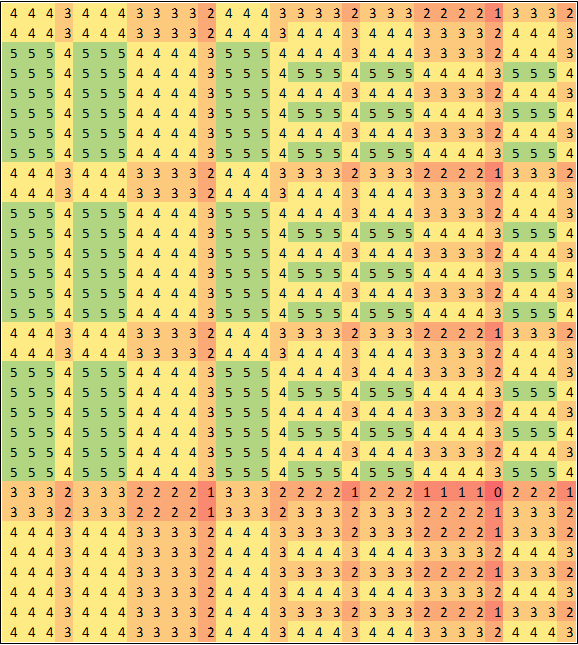
\includegraphics[width=2.5in]{img/D(tacgt)}
			% 	\caption{\small
			% 		Distribution $\mathcal{D}$(\texttt{tacgt}) of Hamming distances from \texttt{tacgt} 
			% 		to all $4^{5} = 32\times32$ $k$-suffixes of length 5.
			% 		The value in the $p^{th}$ cell of this $32\times32$ table (at row $\frac{p}{32}$, col $p$ \emph{mod} 32) is the Hamming distance from the \textbf{center} \texttt{tacgt} to the $k$-suffix that maps to the binary number $p$.
			% 		%, i.e. $D(z)_{p} = dH(z,\emph{unmap}(p))$.\newline
			% 		Ex. $\mathcal{D}(\texttt{tacgt})_{100} = dH(\texttt{tacgt}, \texttt{acgca}) = 5$.\newline
			% 		%$D(\texttt{tacgt})_{24,27} = dH(\texttt{tacgt}, \emph{unmap}(795)) = dH(\texttt{tacgt}, \texttt{tacgt}) = 0$.
			% 	}
			% 	\end{figure}\newline
			% Due to the alphabetical enumeration, the $4^{k}$ $l$-mers grouped together in a block will all begin with the same ($l-k$) characters---the {\boldmath\bf block prefix $y'$}. The block's {\boldmath\bf prefix distance $d_{y'}$} is just the Hamming distance $dH(y,y')$ between $x$'s prefix and the block prefix.\newline\newline
			% 	{\small
			% 		Ex. For block \{\texttt{acgttgcaaaaa} to \texttt{acgttgcttttt}\}\newline
			% 		\hspace*{18pt} the prefix distance from $x$ = \texttt{acgtacgtacgt} is\newline
			% 		\hspace*{21pt} $d_{y'} = dH(\texttt{acgtacg}, \texttt{acgttgc}) = 3$. } \newline\newline
			% We can infer that the distance between any two $l$-mers is equal to the sum of the distance between their prefixes and the distance between their $k$-suffixes; thus, given $d_{y'}$ and $\mathcal{D}(z)$, we can compute the distance from $x$ to any $l$-mer $x' = y'z'$ in a block as:
			% \begin{equation}
			% 	dH(x,x') = d_{y'} + \mathcal{D}(z)_{z'}
			% 	\end{equation}
			% We can now redefine the criteria for setting a bit in $N$:
			% \begin{equation*}
			% 	N_{x'} = \left\{
			% 	\begin{array}{rl}
			% 		1 & \text{if } d_{y'} + \mathcal{D}(z)_{z'} \leq d,\\
			% 		0 & \text{otherwise.}%\text{if } d_{y'} + \mathcal{D}(z)_{z'} > d.
			% 	\end{array} \right.
			% 	\text{ for }x' = y'z'.
			% 	\end{equation*}
			% From this we see that a bit at position $z'$ within a block with prefix $y'$ will be set if and only if $D(z)_{z'} \leq d-d_{y'}$. The values in $D(z)$ range from 0 to $k$; therefore\newline

			% 	{\small
			% 		\hspace*{5pt} when $d-d_{y'} < 0$, 		\hspace*{24pt}no bits in the block are set;\newline
			% 		\hspace*{5pt} when $0 \leq d-d_{y'} < k$,	\hspace*{6.5pt}some bits are set ($k$ ways); and\newline
			% 		\hspace*{5pt} when $d-d_{y'} \geq k$, 		\hspace*{24pt}all bits in the block are set. \newline}
			
			% This allows for ($k + 2$) unique patterns of bits, including ``empty'' (all 0's) and ``full'' (all 1's), for blocks in $N$.\newline
			% \begin{figure}[h]
			% 	\centering
			% 	\label{fig:bit_patterns}
			% 	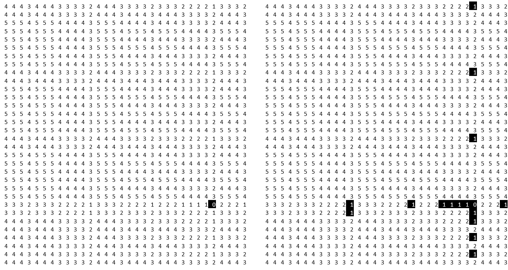
\includegraphics[width=3.1in]{img/0-1}\vspace*{5pt}
			% 	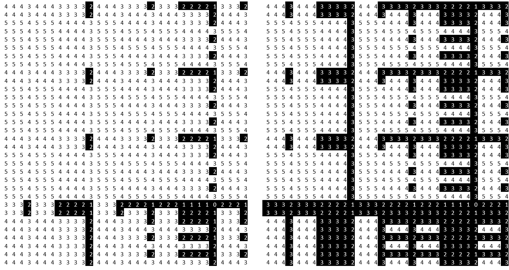
\includegraphics[width=3.1in]{img/2-3}\vspace*{5pt}
			% 	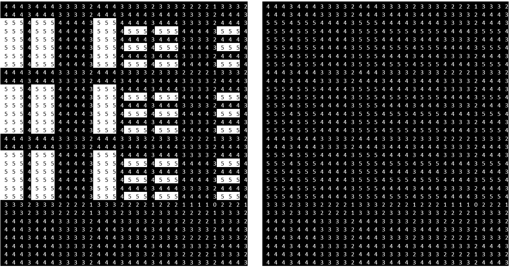
\includegraphics[width=3.1in]{img/4-5}
			% 	\caption{\small Bit patterns followed by blocks of size $4^{5}=32\times32$ in the bit-based representation of $\mathcal{N}(\texttt{acgtacgtacgt},5)$. Black signifies a 1. There are $(5+2)=7$ possible patterns---the empty pattern (all 0s) is not shown.}
			% 	\end{figure}
			% \newpage

	\section{Performance of optimized EMS-GT}
		EMS-GT and two competitor algorithms were run on an Intel Xeon, 2.10 GHz machine. Their performance, averaged over 20 synthetic datasets for each $(l,d)$ challenge instance, is outlined in Table~\ref{tbl:runtimes_v_pms}:\newline

		\begin{table}[ht] %runtimes
			\renewcommand{\arraystretch}{1.3}
			\label{tbl:runtimes_v_pms}
			\centering
			\begin{tabular}{|c|c|c|c|c|}
			\hline \bfseries\boldmath $(l,d)$ & \bfseries PMS8 & \bfseries qPMS9 & \bfseries EMS-GT & \bfseries \% speedup\\
			\hline
			 9,2 &  0.74 s  &  0.47 s & {\bf 0.11 s} & 76.6\%\\
			11,3 &  1.58 s  &  1.06 s & {\bf 0.20 s} & 81.1\%\\
			13,4 &  5.39 s  &  4.52 s & {\bf 1.04 s} & 77.0\%\\
			% 14,4 &  1.29 s  &  1.02 s &      2.55 s\\
			15,5 & 36.45 s  & 24.63 s & {\bf15.51 s} & 37.0\%\\
			% 16,5 &  4.79 s  &  2.96 s &     29.03 s\\
			17,6 &  3.91 min & \textbf{1.96 min} & {\emph{2.93 min}} & --\\
			\hline\end{tabular}

			\caption{Runtimes of PMS8, qPMS9 and EMS-GT}
			\end{table}

		
		For every challenge instance except (17,6) EMS-GT outperforms qPMS9; it outperforms PMS8 for instance (17,6). EMS-GT was run including the block-masking optimization, with the default suffix length of $k$=5. Observe that our EMS-GT implementation can only solve problem instances where $l \leq 17$. This is because when we reach $l$=18, the size of the integer array needed to represent the entire search space ($\frac{4^{18}}{32} = \frac{2^{36}}{2^{5}} = 2^{31}$ integers) begins to exceed the maximum size for Java arrays, which is ($2^{31} - 1$) elements.\newline


\chapter{Conclusions}

%\BackMatter
\bibliographystyle{plain}
\bibliography{sources}
%\addappheadtotoc
%\input{APPENDIX}

\end{document}
